% Chapter Template

\chapter{Technologies Used} % Main chapter title

\label{Chapter2} % Change X to a consecutive number; for referencing this chapter elsewhere, use \ref{ChapterX}

\section{Introduction}
In the previous chapter, we went over an introduction to the context of the work as well as the methods through which we can accomplish the goal of learning the behaviour of the robot as it moves in the configuration space.
As we know a basic introduction to the work,  in this chapter we would go over the technologies that are employed to achieve the goal of learning the behaviour of the robot. We will first go over the hardware and software requirements of the robot, and the environment.
\section{Hardware Employed}
The project uses a Turtlebot2 \cite{t2} robot. Turtlebot2 (see Figure~\ref{fig:Turtlebot2}) is a low-cost, personal robot kit with open-sourced software. The robot was created in 2010, but has been continuously envolved in both 
software strength and hardware with open-source contributions to the project. The Turtlebot2 consists of a base, two wheels, a single board computer and a LIDAR sensor. Other sensors for example a vision sensor, i.e. Camera can be attached later to the mainframe based upon the requirement.
Turtlebot2 accomplishes SLAM and Navigation efficiently in the configuration space. It is developed to be employable in various scenarios, and can be controlled remotely by a computer or a joystick. 
Turtlebot2 can be attached with an arm to perform manipulator tasks.

\begin{figure}[th]
    \centering
    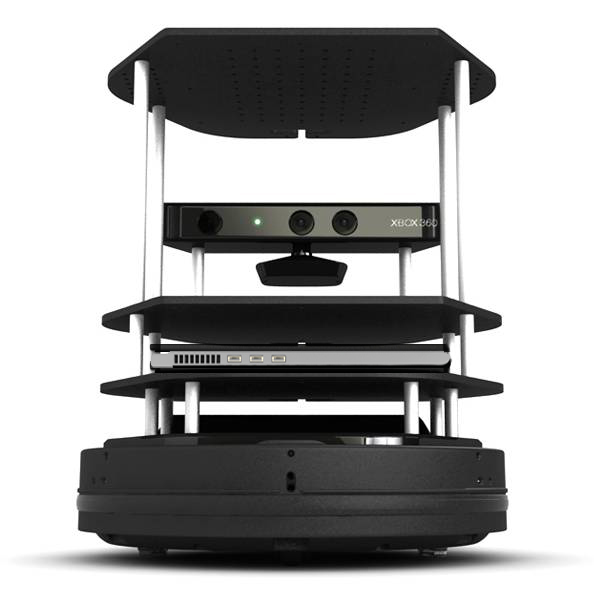
\includegraphics[width=0.5\textwidth]{Figures/turtlebot2.jpg}
    \decoRule
    \caption[]{Turtlebot2}
    \label{fig:Turtlebot2}
    \end{figure}

\subsection{LIDAR Sensor}
LIDAR stands for light detection and ranging. LIDAR sensor measures the time of flight of the pulse of light.
The light transmitted from LIDAR hits an obstacle and is noted. The light transmitted is usually infrared, where most of the energy is concentrated
in a narrow beam of light. The distance to the obstacle is calculated by measuring the time of flight in seconds.
The hardware involved here is a receiver emitter pairs (channels) which is combined wuth rotating mirrors to ensure that the whole area is covered.
They are used in autonomous devices. The sampling rate of a LIDAR is high, therefore the light beams do not collide with one another resulting in precision.
The range of LIDAR sensor are measured by maximum likelihood estimators. There are various types of LIDAR sensors with varying capabilities such as difference in the scanning area, resolution, detection range.
The resuting data collected is a point cloud grid.
\section{Software Employed}
\subsection{Gazebo Simulator}
In the implementation, we are using \textbf{Gazebo} \cite{1389727} as a simulator to visualize and execute the processes.
Gazebo is a well-designed high quality simulation software with a real physics engine. Gazebo makes it easy for researchers to test AI algorithms, design Robots, perform regression and testing and train AI systems before 
using it in real-world applications. Gazebo can use 3D models to implement real-world scenarios for the robot to interact with. It is a trusted simulator, being used by reputed space agencies to simulate robots.
Turtlebot2 has packages for Gazebo to present the robot in simulation. Gazebo's biggest advantage is it's huge community support around it.

Gazebo provides many features:
\begin{itemize}
    \item \textit{Dynamic Simulation : } Simulation is provided by many high-quality physics engine such as ODE, Bullet and DART.
    \item \textit{Advanced 3D Graphics : } Gazebo provides great simulation which is very realistic including textures, lighting and shadows.
    \item \textit{Sensors and Noise :} Simulator can be used to make real sensor data with noise from sensors and other equipments such as laser range finders, vision sensors and contact sensors etc.
    \item \textit{Plugins :} Researcher can develop custom plugin for a specific sensor or a specific task in the simulation.
    \item \textit{Robot Models: } There are many different robots which can be used in Gazebo, from simple robots such as Turtlebot2/3 to Mars Rover can be simulated in a Gazebo environment.
    \item \textit{TCP/IP Transport: } We can run simulation on remote servers, and interface with Gazebo simulator through socket based message pushing.
    \item \textit{Cloud Simulation :} CloudSim can be used to run Gazebo on Amazon Web services, or personal web service or personal architecture.
    \item \textit{Command Line Tools : } Command line tools simplify simulation control and introspection.
\end{itemize}
Gazabo11 was the version being implemented with ROS Noetic in this report's context.

\subsubsection{Environment's Entities}
In Gazebo's simulation, we get presented with a blank environment to build upon. We use Computer Aided Design (CAD) to create required entities and obstacles. In our implementation,
we had to develop boxes, tiles and borders to the environmment. The model is saved in \textit{sde} format, and rendered in Gazebo. Each box is placed at a specific position, and the borders are placed
to enclose the environment. The whole entity is made over a sheet of tile. The Gazebo environment with a turtlebot is demonstrated in the Figure~\ref{fig:GazeboTurtlebot2} 
\begin{figure}[th]
    \centering
    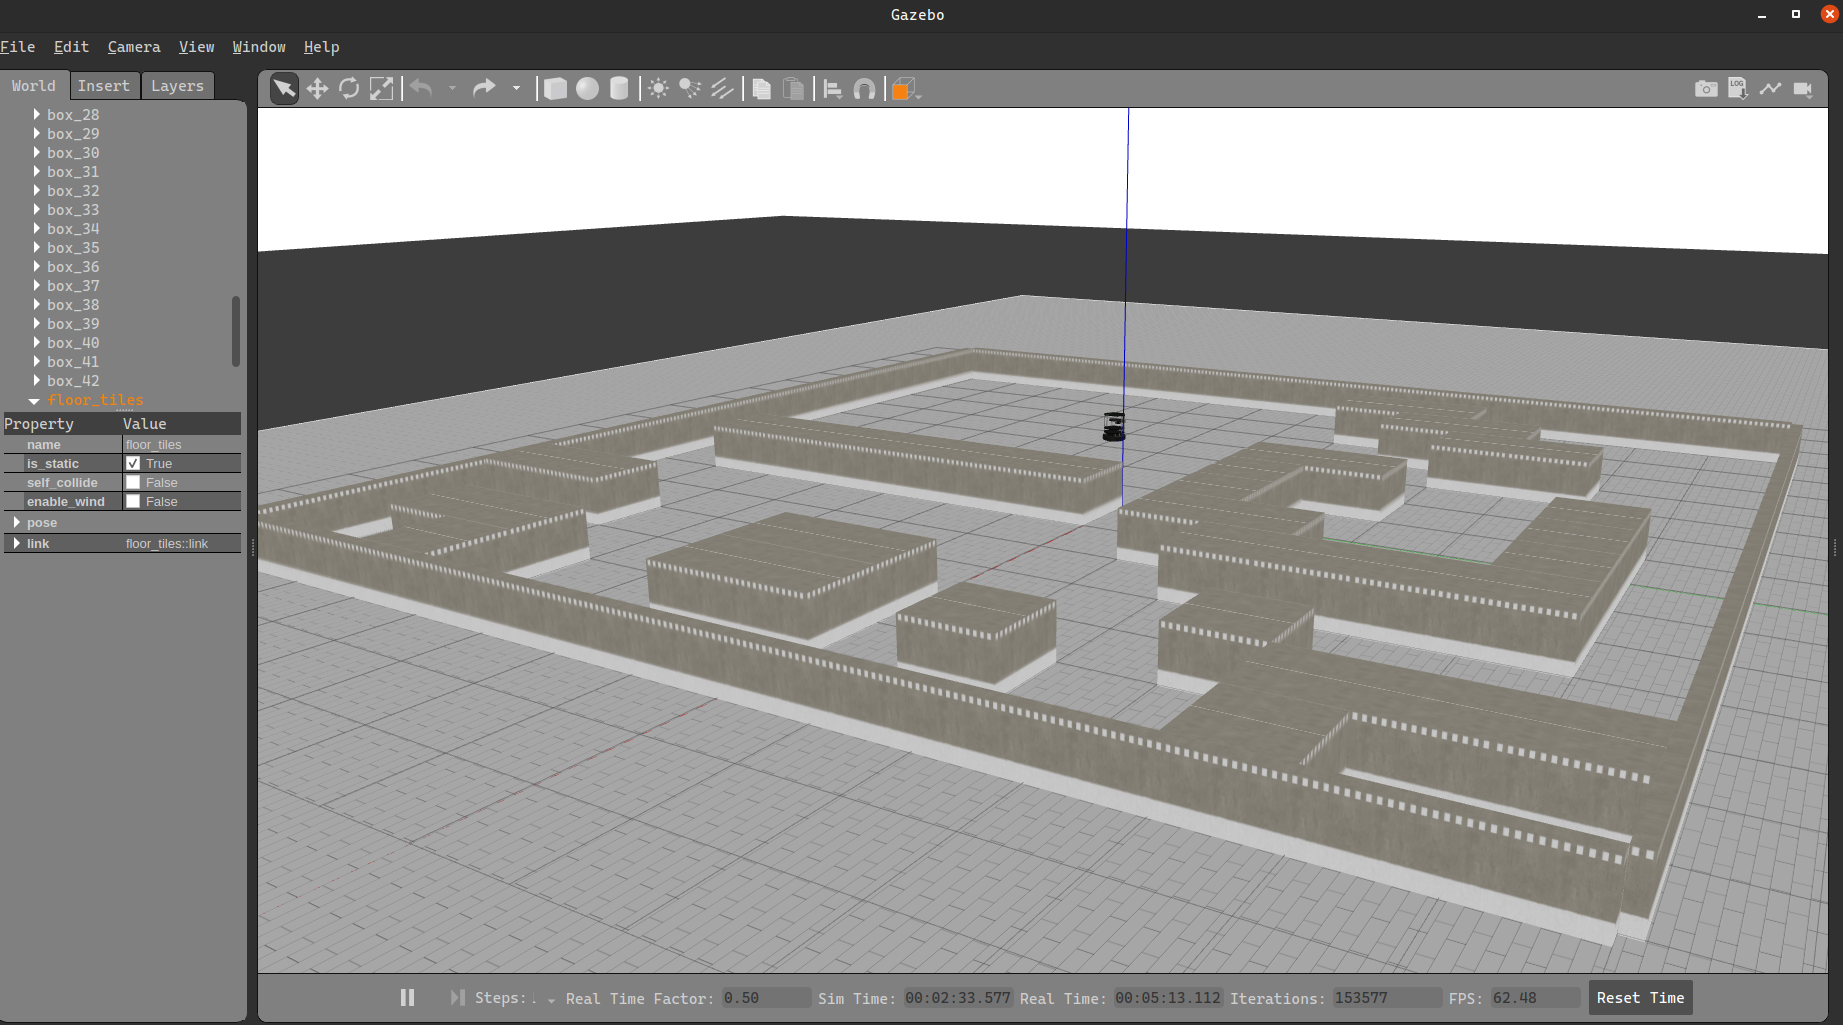
\includegraphics[width=\textwidth]{Figures/gazebo-image.png}
    \decoRule
    \caption[]{Turtlebot2 in Gazebo Environment}
    \label{fig:GazeboTurtlebot2}
\end{figure}

\section{Robot Operating System}
Robot Operating System or ROS, is known for it's flexibility as a framework to write and simulate robot software. ROS has a collection of open-source tools and libraries are used to run robots. It is
very helpful in the field of robotics as it reduces the hassle of writing and figuring most of the robot's driver and actuator code. It is at a higher level in abstraction, thus providing an option to use the same
code in simulation in Gazebo as well as to run the real robot. It provides hardware abstraction, libraries, device drivers, package management and more. 
There are various different versions of ROS, each combined with a specific version of Ubuntu's Long Term Service distribution. As the software we wish to build is supposed to be utilized later, a stable framework is a neccesity. Ubuntu 20.04 LTS and 
ROS Noetic were chosen as distributions for the project.

\subsection{ROS Packages}
In ROS, we have different packages for differnt softwares. A package is created by specific ROS commands. A ROS Package structure is : 
\begin{itemize}
    \item \textit{include/package name}: C++ scripts include headers which are stored in this directory.
    \item \textit{msg} : This folder contain msg types, i.e the types of messages being interchanged in processes.
    \item \textit{src} : This folder contains the source file for the package.
    \item \textit{srv} : This folder contains files which show the simplified service description languages.
    \item \textit{scripts} : This folder contains the scripts (in python) required to run the robot or do a specific task.
    \item \textit{CMakeLists.txt} : This file describes the ROS Package and helps the developer to specify runtime and execution time dependancies to build the catkin project.
    \item \textit{package.xml} : Describe the dependancies of the package.
    \item \textit{CHANGELOG.srt} : Many packages will define a changelog which can be automatically injected into binary packaging and into the wiki page for the package
\end{itemize}

\subsection{ROS Command Line Tools}
Packages are a central concept that are used to manage different software. Some command line tools help you to manage such packages : 
\begin{itemize}
    \item \textit{rospack} : finds and retrieves information about the package.
    \item \textit{catkin-create-pkg} : creates a new ROS package. 
    \item \textit{catkin-make} : build the workspace containing different ROS packages.
    \item \textit{rosdep} : to install the system dependencies of the package.
    \item \textit{rqt} : RQT has a  a plugin called "Introspection/Package Graph", which visualizes package dependencies as a graph.
\end{itemize} 

\section{Simulataneous Localization and Mapping}
As we studied in the previous chapter about localization, which is a process to inform the robot about it's position in the environment it is in. 
Simultaneous localization and mapping (SLAM)
is a technique applied in artificial intelligence mobile robot for
a self-exploration in numerous geographical environment.
SLAM becomes fundamental research area in recent days as it
promising solution in solving most of problems which related
to the self-exploratory oriented artificial intelligence mobile
robot field \cite{7482163}. SLAM is one of the most fundamental part of autonomous mobile robot navigation. It is used by the mobile robot to navigate around the environment 
and generate a map. The map generated is used to find the obstacle location and grid surrounding the robot to make an appropriate path planning scenario for the robot.
Although Localization and Mapping are different technologies, SLAM incorporates them together where localization is done concurrently with the robot creating the map.
The map is used to note than landmark position and be able to generate an efficient path trajectory. SLAM has the advantage of doing this together at the same time making it the most important 
algorithm in autonomous robot navigation. SLAM methods implement Extended Kalman filters. Figure~\ref{fig:SLAMFlowchart} demonstrates the SLAM process.
\begin{figure}[th]
    \centering
    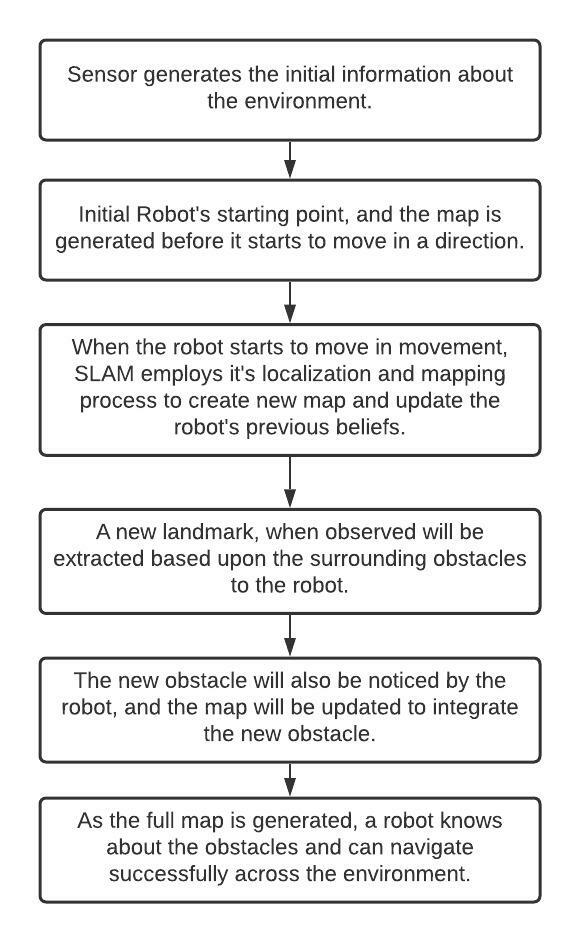
\includegraphics[width=0.5\textwidth]{Figures/SLAM_flowchart.jpeg}
    \decoRule
    \caption[]{SLAM Workflow \cite{7482163}}
    \label{fig:SLAMFlowchart}
\end{figure}
\begin{figure}[th]
    \centering
    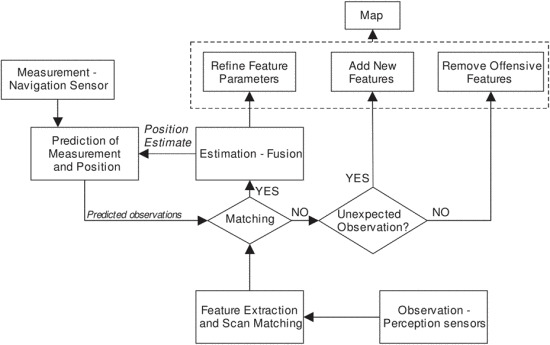
\includegraphics[width=0.8\textwidth]{Figures/SLAM_Block_Final.jpeg}
    \decoRule
    \caption[]{SLAM Block Diagram \cite{7081165}}
    \label{fig:SLAMBlockDiagram}
\end{figure}

\subsection{Features of SLAM}
Three major features of SLAM exist and are discussed below : 
\subsubsection{Mapping}
For a robot to move around autonomously in an environment. It should know where it is, providing prior knowledge. Mapping provides his capability for the robot to generate a map using the hardware sensor (mostly LIDAR) to get information from the environment.
There are various ways to represent the map, which are used to generate a path in subsequent steps. The data will be used by the robot to localize and recognize it's own position and landmark.
\subsubsection{Localization}
Localization is calculated by using the odometry of the robot. It is one of the features of SLAM which are able to calculate and estimate the poisition of the robot, and the obstacles close to it.
The mobile robot should be able to \textit{think} for itself by calculating and estimating the path travelled and calculating the nearby obstacles. 
\subsubsection{Navigation}
Navigation employs both Mapping and Localization, by combining the results of both. When the robot navigates through the environment, mapping and localization process are 
executed periodically and repeatedly recursively to update the robot's information from the environment and saves the map. The robot's exploration is implemented and is able to backtrack to origin point 
or starting position. Path Planning is done with various algorithms, such as Dijkstra, A\textsuperscript{*}, Potential Field and other algorithms. In our implementation, we used different algorithms which we will describe in \ref{planner-algorithms}

\subsection{Isssues in SLAM}
As every method, SLAM has it's owm issues which are uncertainty, correspondence and data association.
\subsubsection{Uncertainity}
There are both location and hardware uncertainity in SLAM which affect the performance of robot while performance. Uncertainity in location determines how capable the robot is to handle multiple paths in environment's location. For a robot
to move in a linear direction, and come back to the same position, the path planning is very easy without any uncertainty because simplicity in motion. In real world, as well as in our implementation the robot is subjected to different paths in the environment.
Therefore, in this case location's uncertainity as well as the final trajectory of the path is often tough and included with a degree of uncertainity. Inaccurate information can be corrected in the post treatment of the data and processed to recognize the robot and obstacles nearby.
\subsubsection{Correspondence}
Identification of the obstacles in the environment is a problem in SLAM. If we consider two different obstacles, with similar shapes but one obstacle is slightly bigger than the other in height, the light radiated from the obstacle when LIDAR will hit shows the same obstacle for both. In such cases, SLAM is not able to update robot's map.
\subsubsection{Data Association}
In data association issues, the SLAM is not accurate in returning to it's original point and previously mapped area. Data association processes are used to estimate the odometry frame of the mobile robot to backtrack from where it came from i.e, it's original state and nearby obstacles.
\subsubsection{Time Complexity}
This issue deals with implementation of SLAM algorithms and methods employed to calculate and compute the information received from the sensors. In 
SLAM the process of localization and mapping are carried out together recursively during navigation in a direction. The processes are executed concurrently in a very short amount of time, the handling and management of the values from the sensors are not managed and calculated efficiently. 
Therefore the performance and time complexity are important to produce reliable results for the robot to explore the environment.

\section{Path Planning Methods}
The previous chapter has introduced the term \textit{motion planning} and \textit{path planning} to us. Path plannng algorithms are used to take the design of the workspace and obstacle space to return the path. The robot follows the path which is returned by the algorithm.
A such algorithm is called a \textit{planner}. According to Steven M. LaValle's definition of a planner \cite{lavelle} : "A planner simply constructs a plan and may be a machine or a human. If the planner is a machine, it will
generally be considered as a planning algorithm. In many circumstances it is an algorithm
in the strict Turing sense, however, this is not necessary. In some cases, humans become
planners by developing a plan that works in all situations"

There are two types of path planning algorithms : 
\begin{itemize}
    \item Global Planner Algorithms
    \item Local Planner Algorithms
\end{itemize}

\subsection{Global Planner Algorithms}\label{planner-algorithms}
Global Path Planner utilises the definition of configuration space of the robot which is based upon the global map.
The global path planning algorithms are known as offline algorithms because the calculation of path is done before the robot moves. Robot's configuration space is used to calculate a path to the final state.
ROS is utilized to convert the map file which was generated by SLAM to divide the map into square boxes and classifying 
them into either obstacle or a free configuration space.

\subsubsection{General Idea}
After SLAM, the made map file is generated and provided to the navigation stack to describe the configuration space.
ROS uses the concept of global costmaps to divide the map into squares based upon it's resolution and the value to each square given in the range of 0-255.
0 signifies a free space while any value greater than one is an obstacle space. We use this information to decide and calculate the path taken by our robot to reach the goal.
Thus, after describing the configuration space we will use Graphs to calculate a viable path to the final destination of the robot.
There are different paths to consider at each and every node in the graph. A path is considered if and only if, a particular next node provides the minimum cost or a user/task specific requirement.
Different Algorithms we implemented in the project provide a different method to solve this problem and predict the next states of the robot to follow.
Figure~\ref{fig:PPGrid} shows all the possible paths to reach the goal.
\begin{figure}[th]
    \centering
    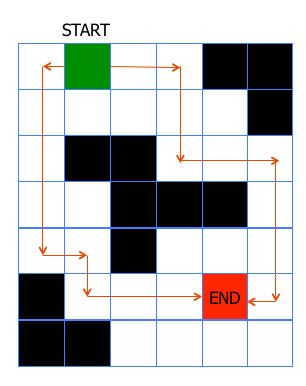
\includegraphics[width=0.5\textwidth]{Figures/grid-path-planning.png}
    \decoRule
    \caption[]{Path Planning Grid}
    \label{fig:PPGrid}
\end{figure}

\subsubsection{Dijkstra Algorithm}
Dijkstra's algorithm is a very generic way to find the path to the goal node which are connected by edges if we consider the configuration space to be a graph. Dijkstra's algorithm was developed by Edsger W. Dijkstra \cite{enwiki:1039157161}. The algorithm
was proposed to solve the path planning by finding the minimum cost path.
\subsubsection{A\textsuperscript{*} Algorithm}
A\textsuperscript{*} algorithm is pretty similar to Dijkstra's algorithm but it has increased performance. Dijkstra's algorithm is a new approach as it starts to explore the global obstacle grid with a starting node and doesn't stop till it reaches the ending node.
It will identify the list of nodes which connect the end node to the starting node to form a path. But there is an issue with Dijkstra, which requires it to explore all the nodes in an equal fashion. This is fine if computation speed and space is not a requirement. 
But exploring all the nodes equally increases the time complexity of the algorithm. If the map is big, using Dijkstra's algorithm can be very computationally expensive. We use A\textsuperscript{*} algorithm to improve the efficiency of search and finding the path.
A\textsuperscript{*} does this by introducing the concept of a \textit{heuristic function} which will help the node exploration towards the goal. The function calculates a correlation of the node to a cost value (a positive value). 
Heuristic functions are calculated by satisfying these basic criteria.

\begin{itemize}
    \item H(goal) = 0
    \item H(x) $<=$ H(y) + cost(x,y), where cost(x,y) is the cost to travel from one node to the other and x,y are the two adjecent nodes. 
\end{itemize}

By keeping the cost of the goal node 0, it helps us increase the cost efficiency because we do not have a direction. Thus, if the cost of travelling from a node to the other can bring us closer to the goal we use it as it increases our exploration time.
Heuristic function cost(x,y) can be calculated by using either Euclidian Distance or Manhattan Distance depending on one's preference. 
\subsubsection{Greedy Best First Search Algorithm}
Greedy Best-First Search (Greedy Best-First Search) Algorithm is a search algorithm. The configuration space is represented as a graph of different nodes. 
The algorithm will explore the whole graph by expanding the nodes which can have promising next nodes according to a rule. Pearl J. \cite{pearlJ} defines GBFS
as an estimation of the most promising next node N by a heuristic evaluation function \textit{f(n)} which, in general, depends on the description of N, the information 
of the goal, the information gathered by the process upto this point, and other knowledge about a problem domain.
Configuration space for GBFS algorithm is accomplished by using Visibility Graph Method. The method states that the path is defined as a line connecting the starting
configuration with the ending goal configuration by employing the non-free configuration space. As we define the non-free configuration paths, possible non-collision paths between the start and goal positions are defined too.
As the information about the robot's workspace increases, the quality of the algorithm increases too. The algorithm will work better when we have much more information about the robot's workspace.

\subsection{Local Planner Algorithms}
Local Planners are dynamic path planning algorithm, which means that the algorithm works online while the robot is moving, unlike global planner algorithms where the next states are already decided and the robot follows the specific path. 
Local Planner Algorithms require constant update and calculation of the values recieved from sensors, wheather it is a LIDAR sensor or a camera vision sensor. The algorithm computes those values returned to predict a short term relapse path towards the goal.
There are several local planner algorithms such as \textit{Dynaamic Window Approach (DWA) local planner}, \textit{Time-Elastic-Band (TEB) local planner} already implemented in the ROS package, which we will discuss about in this section. Local Planner also helps the robot to maintain it's path that was calculated earlier by the global planner algorithm. 
In this subsection, we will discuss about the local path planning algorithms.

\subsubsection{TEB local planner}
Configuration space's representation in TEB local planner is done by using a \textit{Sampling-Based approach}.
The planner uses a novel approach named \textit{Time-Elastic-Band algoritm} for obstacle avoidance purposes.The algorithm is described
in the paper \cite{KELLER20149822}. The motion planning is to move the robot from A(x\textsubscript{o}, y\textsubscript{o}) to B(x\textsubscript{N}, y\textsubscript{N}) without any collision with relation to the global and local reference frames.
The local path planner provides a turn in the angle of rotation in \textit{y} axis and a forward motion to avoid the obstacle. 

TEB (see Figure~\ref{fig:TEBPlanner}) is done by describing a fixed number of points to the final goal, \textit{(x\textsubscript{0}, y\textsubscript{0})}, \textit{(x\textsubscript{1}, y\textsubscript{1})}, \textit{(x\textsubscript{2}, y\textsubscript{2})}\dots \textit{(x\textsubscript{N}, y\textsubscript{N})}
 . The different points are put apart by a time interval. The time interval is the difference in travelling two points. Time Elastic Band is made up from 
two different set of points and the time interval, i.e B = (Q,T) and the time band is computed by minimizing a sum of multiple objectives and cost functions to find the new path to get to the final position. The differences betweent the consecutive points are used to calculate the velocity and acceleration for the robot.

\subsection{DWA local planner}
DWA local planner (see Figure~\ref{fig:DWAPlanner}) stands for using \textit{Dynamic Window Approach} to navigation in a regular updating fashion on the surface. After the global path planner gives a path and a costmap configuration space, the local planner will send the velocity to the robot to avoid any obstacles.
DWA local planner utilises the BaseLocalPlanner interface which is specified in the navigation package. The \textit{dwa local planner} provides a controller to control the mobile motor of the robot. The controller will connect the path planning process to the robot. The robot uses a map to create a planner trajectory to get from the start to goal location.
Grid is created around the robot using the LIDAR sensor. The grid cells are utilized to calculate cost value, and the controller will use utilize the value function to send the values of velocity\textsubscript{x}, velocity\textsubscript{y} and velocity rotation theta to the robot.

Major ideas in Dynamic Window Approach (DWA) are described below : 
\begin{itemize}
    \item Getting values from robot's LIDAR sensor and discretely calculating the robot's control space.
    \item Velocity is calculated from the function to calculate the current state and predicting the next sampled velocity with next state in case of deflection with an obstacle.
    \item The velocity will be applied for a very short period of time.
    \item Different trajectories are generated to avoid the obstacle.
    \item The trajectory with the highest score and providing the lowest cost to move towards the goal is chosen.
    \item The trajectory is chosen, and the associated velocity is sent to the motor by the controller. 
    \item You repeat the algorithm everytime you find an obstacle. 
\end{itemize}

Our choice was to use Dijkstra algorithm for the global planner algorithm and dynamic window approach for the local planner algorithm.
Implementation for A\textsuperscript{*} and GBFS algorithm is also done, and can be implemented based upon preference.

\begin{figure}[th]
    \centering
    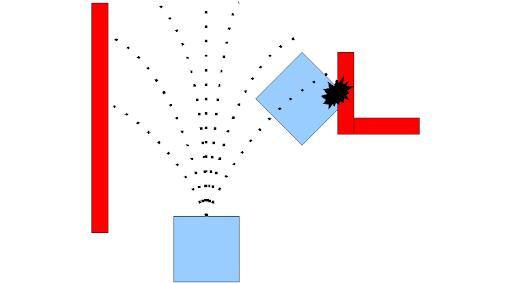
\includegraphics[width=0.9\textwidth]{Figures/dwa_planner.png}
    \decoRule
    \caption[]{DWA Planner}
    \label{fig:DWAPlanner}
\end{figure}

\begin{figure}[th]
    \centering
    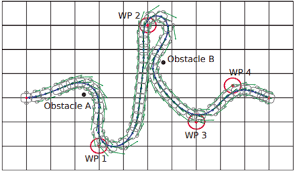
\includegraphics[width=0.9\textwidth]{Figures/TEB.png}
    \decoRule
    \caption[]{TEB Planner}
    \label{fig:TEBPlanner}
\end{figure}


